\documentclass[pageno]{jpaper}

\usepackage{hyperref}
\usepackage{url}
\usepackage{setspace}
\usepackage{amsmath}
\usepackage{amssymb}
\usepackage{clrscode3e}
\usepackage{makecell}
\usepackage{listings}
\usepackage{xcolor}

\newcommand{\IWreport}{Spring 2025}
\newcommand{\quotes}[1]{``#1''}

\definecolor{codegreen}{rgb}{0,0.6,0}
\definecolor{codegray}{rgb}{0.5,0.5,0.5}
\definecolor{codepurple}{rgb}{0.58,0,0.82}
\definecolor{backcolour}{rgb}{0.95,0.95,0.92}
\newcommand\iid{i.i.d.}
\lstdefinestyle{mystyle}{
    backgroundcolor=\color{backcolour},   
    commentstyle=\color{codegreen},
    keywordstyle=\color{magenta},
    numberstyle=\tiny\color{codegray},
    stringstyle=\color{codepurple},
    basicstyle=\ttfamily\footnotesize,
    breakatwhitespace=false,         
    breaklines=true,                 
    captionpos=b,                    
    keepspaces=true,                 
    numbers=left,                    
    numbersep=5pt,                  
    showspaces=false,                
    showstringspaces=false,
    showtabs=false,
    tabsize=4
}

\lstset{style=mystyle}

\newcommand{\xmin}{x_{\textrm{min}}}
\newcommand{\xmax}{x_{\textrm{max}}}
\newcommand{\ymin}{y_{\textrm{min}}}
\newcommand{\ymax}{y_{\textrm{max}}}
\newcommand{\fmin}{f_{\textrm{min}}}
\newcommand{\fmax}{f_{\textrm{max}}}
\newcommand{\fminb}{f_{\textrm{min\_bound}}}
\newcommand{\fmaxb}{f_{\textrm{max\_bound}}}

\makeatletter
\def\verbatim@font{\linespread{1}\normalfont\ttfamily}
\makeatother

\graphicspath{ {./images/} }

\begin{document}

\title{
Robustness Verification for Ensemble Learning Methods
}
\author{Samuel Sanft\\Adviser: Aarti Gupta}
\date{}
\maketitle

\begin{doublespacing}

\begin{abstract}
This paper proposes a new method for verifying local robustness of decision tree-based ensemble learning methods. It proposes a data structure for representing these models and algorithms for merging and pruning decision trees, which can be used to set lower and upper bounds on the output of a model. These algorithms can be used in conjunction with existing optimization techniques to verify or disprove local robustness. This method can be applied to common ensemble methods including bagging, random forests, and gradient boosted models. This paper demonstrates how the proposed method outperforms current satisfiability modulo theory (SMT)-based methods for local robustness verification by several orders of magnitude. It also attempts to use this method to compare the effect of model choice and model size on local robustness in both regression and classification settings.
\end{abstract}

\section{Introduction}
Robustness verification is an important, yet challenging problem in the field of AI safety. Local, or adversarial, robustness refers to a trained models performance, when small perturbations are introduced to the input data. Non-robust models may drastically alter their predictions when the input data is very slightly perturbed (see \autoref{fig:noisy1}). This can negatively impact the performance of a model, when random noise is introduced. Non-robust models are also susceptible to adversarial inputs, which are designed to cause misclassification, despite very closely resembling properly classified inputs. Performing robustness verification on decision tree-based ensemble methods, such as random forests or gradient-boosted tree models, is a challenging task, since these models are non-continuous and non-differentiable. This means that verification techniques used for other models, such as neural networks, generally can't be employed. However, these models remain incredibly popular, due to their ease of training and state of the art performance on a multitude of tasks. This means that the challenge of efficient and accurate robustness verification for decision tree-based ensembles remains an open and compelling problem.

%%%%%%%%%%%%%%%%%%%%%%%%%%%%%%  Background  %%%%%%%%%%%%%%%%%%%%%%%%%%%%%%
\section{Background Work}
\subsection{Decision Trees}
Decision trees are a common statistical and machine learning model that can be applied to both regression and classification learning tasks \cite{james}. Decision trees partition the feature space into distinct regions and predict a singular outcome for each region. Each splitting node of a tree selects a single feature axis and an associated numeric threshold, and points to left and right subtrees (throughout this paper, decision trees will exclusively refer to binary decision trees and the threshold will alway be a real value). For example, a splitting node may have axis $k$ with threshold $c$. In this case, inputs processed by this node where $x_k \le c$ will be sent to be processed by the left subtree, while inputs where $x_k > c$ are processed by the right subtree. Each leaf of a decision tree represents a region of the feature space and predicts a value meant to approximate the target function over that region. In the regression case this is a numeric value (for this paper it will always be considered as a real number), while in the classification case each leaf will predict a vector of probabilities, one for each distinct label class, whose entries are nonnegative and sum to 1. The predicted class is the entry with the largest probability, and the greater the probability, the higher the models confidence in the prediction. A decision tree predicts an outcome for an input $x$ by starting at the root node and traversing down the tree following the decision procedure described above until a leaf node is reached. Both classification and regression trees are typically trained using the CART algorithm \cite{breiman1984}.

\subsection{Ensemble Methods}
While singular decision trees are often poor predictors for more complex learning tasks, due to their tendency for overfitting and overall poor generalizability, ensembles of decision trees can be employed which typically demonstrate much better predictive performance. An ensemble of decision trees produces a prediction by averaging the predictions of each individual tree within the ensemble. In the classification case, the probability vectors of each decision tree are averaged and the predicted label class is the label class with the largest probability. An ensemble can be formally defined as follows, where $f$ represents the whole ensemble, $f_i$ represents a singular decision tree, and $B$ is the total number of trees in the ensemble:

$$f(x) = \frac{1}{B} \sum_{i=1}^N f_i(x)$$

There are multiple types of decision tree-based ensemble methods, that differentiate themselves in the way that they train their individual trees. In this paper, three common methods will be examined: bagging, random forests, and gradient-boosted trees.

\subsubsection{Bagging}
Bagging refers to bootstrap aggregating and is a simple way of reducing the variance of a decision tree based learning model by training many decision trees that are correlated with each other \cite{breiman1996}. This is done by generating many bootstrapped samples of the training data. A typical training dataset will be composed of features and labels, $D = \{ (x^{(n)}, y^{(n)}), n = 1, \cdots, N \}$. A bootstrapped sample $D^{(b)}$ is a dataset containing $N$ samples from $D$, drawn randomly with replacement. In order to train a bagging model, $B$ bootstrapped datasets are generated. One decision tree is trained for each bootstrapped sample $D^{(b)}, b=1, \cdots, B$, and the resulting ensemble produces predictions by averaging over all trees.

\subsubsection{Random Forests}
Random forests are an extension to bagging \cite{breiman2001}. In addition to training each decision tree on an independent bootstrapped sample of the training data, only a random subset of the features are allowed to be considered at each splitting node within each tree. This typically leads to greater diversity among the feature selection within the splitting nodes which can reduce variance and lead to better generalizability when averaged across many trees.

\subsubsection{Gradient-boosted Trees}
Gradient-boosted trees train decision trees iteratively by fitting a decision tree to the current residuals \cite{friedman}. Typically a learning rate $\lambda$  is employed to slow down training and prevent overfitting. For example at iteration $b$, the model is defined:
$$f^{(b)}(x) = \lambda \sum_{i = 1}^b f_i$$

The residuals at iteration $b$ are defined:
$$r_b^{(n)} = y^{(n)} - f^{(b)}(x^{(n)})$$

Decision tree $f_{b + 1}$ is then trained on the modified dataset $D^{(b)} = \{ (x^{(n)}, r_b^{(n)}), n = 1, \cdots, N \}$. The training process is usually stopped once a fixed number of trees have been trained, or the residuals become too small. Unlike bagging and random forests, which typically use fully trained decision trees (meaning each tree is grown until it can perfectly or near perfectly predict it's own training data), gradient boosting typically sees best results when the individual trees are limited either in depth or in total size.

\subsection{Robustness Verification}
Local robustness refers to a learning model's robustness against small perturbations in the input data. These perturbations could be due to random noise or adversarial inputs. This paper uses a similar definition for local robustness as \cite{einziger}, \cite{katz}. Formally, a regression model $f$ is $(\epsilon, \delta)$-robust at a location $x$, if for all inputs $x'$ such that $||x - x'||_\infty \le \delta$, $|f(x) - f(x')| \le \epsilon$. A classification model $f$ is $\delta$-robust at a location $x$, if for all inputs $x'$ such that $||x - x'||_\infty \le \delta$, $f(x) = f(x')$ (where $f(x)$ is the predicted label class, rather than the vector of predicted probabilities). Although local robustness can only be proven at individual locations, the percentage of samples that are locally robust from a representative distribution (such as a testing or validation dataset), can be used as a benchmark of a models general robustness.

\autoref{fig:noisy1} depicts an example of a non-robust sample, from a random forest model trained on the MNIST dataset of hand-drawn digits \cite{mnist}. By only slightly varying the brightness of the pixels (enough to just barely be perceptible to a human), the model goes from predicting that the image is a 1 with 98\% probability, to predicting that the image is a 2 with 79\% probability. Although local robustness can apply to any type of machine learning model, computer vision and image recognition tasks are a common application, as it is easy for a human to observe how very slight changes to the input can drastically affect the output of a model.

\begin{figure}[h]
\centering
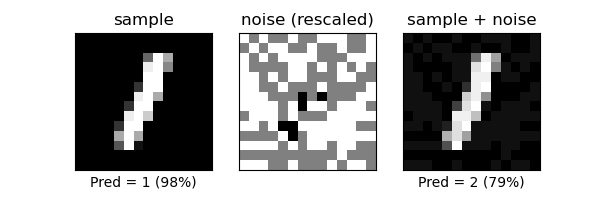
\includegraphics{noisy_1}
\caption{Non-robust sample from Random Forest}
\label{fig:noisy1}
\end{figure}

Many methods have been proposed for performing robustness verification on various types of machine learning models. \cite{katz}, \cite{wu} present efficient methods for verifying local robustness of neural networks, using convex relaxations of activation functions. \cite{kantchelian} demonstrates that robustness verification for general decision-tree ensembles (meaning that input dimension, tree size, and number of trees are unbounded) is an NP-Complete problem. \cite{chen} refines this complexity characterization by reducing the problem to max-clique enumeration, showing that linear time algorithms exist for single trees and that polynomial time algorithms exist for low-dimensional models. \cite{tornbloom} demonstrates that some local robustness queries can be proven efficiently by setting bounds on the outputs of a model. This is done by averaging the minimum leaf values of every tree in an ensemble to obtain a lower bound for all outputs of the ensemble, as well as averaging the maximum leaf values to obtain an upper bound. However, this method is not always able to prove robustness. \cite{einziger}, \cite{nie} present methods for verifying robustness of random forests and gradient boosted models, respectively, by encoding the model and the local robustness property as a satisfiability modulo theory (SMT)-formula and using an SMT solver. This method works very well for smaller models but scales poorly as the size of the model increases.

\subsection{Particle Swarm Optimization}
Particle swarm optimization (PSO) is an iterative optimization algorithm inspired by the movement of groups of animals such as flocks of birds or schools of fish \cite{kennedy}. Let $f: \mathbb{R}^p \rightarrow \mathbb{R}$ be the cost function to be minimized. Let $b_{l}, b_{u} \in \mathbb{R}^p$ be the lower and upper bounds of the search space, respectively. The swarm is represented by a set of particles $X \in \mathbb{R}^{N \times p}$ that is sampled from the uniform distribution $U(b_l, b_u)$ at initialization. Initialize the velocity for each particle $v^{(n)}$ to 0. For each particle $x^{(n)}$, keep track of it's best known position that it's visited so far $p^{(n)}$. Let $p^*$ be the best position found by the swarm, or $\arg \min_{p \in \{ p^{(1)}, \cdots, p^{(N)} \}} f(p)$. At each iteration, calculate each particles velocity by $v^{(n)} \leftarrow \rho v^{(n)} + w_p r_p^{(n)} (p^{(n)} - x^{(n)}) + w_s r_s^{(n)} (p^* - x^{(n)})$, where $\rho, w_p, w_s$ are hyperparameters and $r_p^{(n)}, r_w^{(n)}$ are uniformly sampled from the range $[0, 1]$ each iteration. Intuitively, $\rho$ represents a particles momentum, $w_p$ represents a pull towards $p^{(n)}$, and $w_s$ represents a pull towards $p^*$. Next, the positions are updated by $x^{(n)} \leftarrow x^{(n)} + v^{(n)}$. After updating the positions, the cost function $f$ is evaluated at the position of each particle, and $p^{(n)}, p^*$ are updated if necessary. The algorithm terminates after a fixed number of iterations, and returns $p^*, f(p^*)$, as the best found solution and value, respectively.

There are a number of hyperparameters that can affect the performance of PSO including the size of the swarm $N$, the momentum factor $\rho$, the pull towards a particle's best known position $w_p$, the pull towards the swarm's best known position $w_s$, and the total number of iterations $T$. PSO is a very flexible optimization algorithm as the underlying function $f$ does not need to be differentiable or even continuous. Normally, the limiting factor in terms of run time is the computation required to evaluate $f$. This makes it a suitable candidate for optimizing the outputs of decision trees or decision tree ensembles, since they are discontinuous but can be evaluated efficiently.

\section{Goals}
This paper presents a new method for performing robustness verification on decision tree-based ensembles that combines the minimum and maximum bound method presented by \cite{tornbloom} with two new algorithms for pruning and merging decision trees in order to verify robust samples. It also employs PSO to find counter-examples for non-robust samples. This method is sound, meaning that when it proves a local robustness query, it has proof of correctness, and when it disproves a query it provides a valid counterexample. However, it is not complete, meaning that in some cases, it may fail to provide an answer. This paper will cover the theoretical approach used to develop this method and briefly cover some details of its implementation. It will also compare the performance of this verification method to the SMT approach proposed by \cite{einziger}, \cite{nie}, as well as use this method to compare the effect of ensemble choice and tree depth on local robustness, across multiple datasets.

%%%%%%%%%%%%%%%%%%%%%%%%%%%%%%  Approach  %%%%%%%%%%%%%%%%%%%%%%%%%%%%%%
\section{Approach}
In order to prove a $(\epsilon, \delta)$-robustness query at a point $x$, one must demonstrate that $f(x) - \epsilon \le f(x') \le f(x) + \epsilon$, when $||x - x'||_\infty \le \delta$. While calculating the minimum and maximum values of an ensemble of decision trees is an NP-Complete problem, calculating the minimum and maximum outputs of a single decision tree can be done efficiently by finding the minimum and maximum values among its set of leaves. We can set a lower bound on $f(x')$ by averaging the minimum values of every decision tree within $f$'s ensemble and an upper bound on $f(x')$ by averaging the maximum values of every decision tree within $f$'s ensemble. Formally:
$$\fminb = \frac{1}{N} \sum_{i=1}^N \min_{x'} f_i (x'), \fmaxb = \frac{1}{N} \sum_{i=1}^N \max_{x'} f_i (x')$$

This paper will refer to $\fminb, \fmaxb$ as the outer bounds, since $\fminb \le \min_{x'} f(x') \le \max_{x'} f(x') \le \fmaxb$. A robustness query can therefore be proven by demonstrating that $f(x) - \epsilon \le \fminb \le \fmaxb \le f(x) + \epsilon$ (this is equivalent to the approach presented by \cite{tornbloom}). A robustness query can be disproven by providing an input $x'$, such that $||x - x'||_\infty \le \delta$ and either $f(x') < f(x) - \epsilon$ or $f(x') > f(x) + \epsilon$.

For simplicity, all robustness queries will be treated as two seperate queries: a minimum query and a maximum query. A minimum query can be proven by showing that $f(x) - \epsilon \le f(x')$, for any $x'$ such that $||x - x'||_\infty \le \delta$, while a maximum query can be proven by showing that $f(x') \le f(x) + \epsilon$, for any such $x'$. A robustness query can be proven by proving its corresponding minimum and maximum queries, while it can be disproven by disproving either one.

This paper proposes a pruning algorithm and a merging algorithm that can be used to refine the outer bounds in order to successfully prove a robustness query. It also describes how PSO can be used to find counterexamples in order to disprove a query.

\subsection{Decision Tree Algorithms}
\label{sec:algorithms}
\subsubsection{Prune}
The proposed pruning algorithm prunes the branches of a decision tree that are unreachable, given an input $x'$, such that $||x - x'||_\infty \le \delta$. It does so by successively applying \verb|pruneLeft| and \verb|pruneRight| to a decision tree along each axis. Given a decision tree, an axis $k$, and a constant $c$, \verb|pruneLeft| removes any branches that are unreachable when $x_k \le c$ while \verb|pruneRight| removes any branches that are unreachable when $x_k \ge c$. Given $x$ and $\delta$, a decision tree can be pruned by successively calling \verb|pruneLeft| on every axis $k$ with $c = x_k + \delta$ and \verb|pruneRight| on every axis $k$ with $c = x_k - \delta$. 

Pseudo-code for \verb|pruneLeft| is provided below. It is a recursive algorithm that traverses along the structure of the tree, starting at the root. The code for \verb|pruneRight| follows the same pattern, but if \verb|axis == tree.axis| it drops the left subtree and prunes the right subtree when \verb|c >= tree.threshold| and prunes only the left subtree while keeping the right subtree intact otherwise.

{\singlespacing
\begin{lstlisting}[language=Python, caption=pruneLeft algorithm]
pruneLeft(tree, axis, c):
	if tree.isLeaf:
		# Don't prune leaves
		return tree

	if axis != tree.axis:
		# Prune both subtrees
		l = pruneLeft(tree.left, axis, c)
		r = pruneLight(tree.right, axis, c)
		return Split(l, r, tree.axis, tree.threshold)

	if c <= tree.threshold:
		# Drop right subtree, prune left subtree
		return pruneLeft(tree.left, axis, c)
	else:
		# Prune only right subtree
		r = pruneLeft(tree.right, axis, c)
		return Split(tree.left, r, tree.axis, tree.threshold)		
\end{lstlisting}
}

\verb|pruneLeft| and \verb|pruneRight| both run in linear or sublinear time, with respect to the size of a tree, since they don't visit any node more than once. When only a small percentage of the samples within the training dataset are contained within the range $[x - \delta, x + \delta]$, applying this procedure can significantly reduce the size of a decision tree. 

By removing any branches of a decision tree that are unreachable when $||x - x'||_\infty > \delta$, it is possible to improve the outer bounds $\fminb, \fmaxb$. Applying this procedure to every tree in an ensemble can also make further analysis significantly more efficient, thanks to a reduction in size of the model. The \verb|pruneLeft| and \verb|pruneRight| algorithms are also a key component of the \verb|merge| algorithm.

\subsubsection{Merge}
The proposed merge algorithm takes two trees $f_1, f_2$ as input and produces a new tree as output $f'$, such that $f'(x) = f_1(x) + f_2(x)$ for any $x$. It is a recursive function that traverses the structure of both trees. Since $\min_x f_1 (x) + \min_x f_2 (x) \le \min_x (f_1 (x) + f_2 ( x))$ and $\max_x (f_1 (x) + f_2(x)) \le \max_x f_1 (x) + \max_x f_2 (x)$, we can narrow the outer bounds by successively applying \verb|merge| to pairs of trees within an ensemble. This reduces the total number of trees within the ensemble, although it may significantly (in certain cases, exponentially) increase the size of each tree.

Partial pseudo-code for the \verb|merge| algorithm is provided below. \verb|addConst| returns a copy of a tree, where each leaf value has been modified by adding a given constant.

{\singlespacing
\begin{lstlisting}[language=Python, caption=merge algorithm]
merge(tree1, tree2):
	# If one or both trees are a leaf, add value to all leaves in other tree
	if tree1.isLeaf:
		return addConst(tree2, tree1.val)
	if tree2.isLeaf:
		return addConst(tree1, tree2.val)

	# Trees split on seperate axes at top node
	if tree1.axis != tree2.axis:
		l = mergeTrees(tree1.left, tree2)
		r = mergeTrees(tree1.right, tree2)
		return Split(l, r, tree1.axis, tree1.threshold)
	
	# Trees split on same axis
	axis = tree1.axis
	t1 = tree1.threshold
	t2 = tree2.threshold
	if t1 < t2:
		l = merge(tree1.left, pruneLeft(tree2.left, axis, t1))
		c = merge(pruneLeft(tree1.right, axis, t2), pruneRight(tree2.left, axis, t1))
		r = merge(pruneRight(tree1.right, axis, t2), tree2.right)
		return Split(l, Split(c, r, axis, t2), axis, t1)
	else if t2 < t1:
		l = merge(pruneLeft(tree1.left, axis, t2), tree2.left)
		c = merge(pruneRight(tree1.left, axis, t2), pruneLeft(tree2.right, axis, t1))
		r = merge(tree1.right, pruneRight(tree2.right, axis, t1))
		return Split(l, Split(c, r, axis, t1), axis, t2)
	else:
		l = merge(tree1.left, tree2.left)
		r = merge(tree1.right, tree1.right)
		return Split(l, r, axis, t1)
\end{lstlisting}
}

In cases where the two trees have no two nodes in common that split along the same axis, the number of leaves in the resulting merged tree is equal to the product of the numbers of leaves in \verb|tree1| and the number of leaves in \verb|tree2|. However, when the trees have some correlation in their structure (which is generally expected to be true for any two trees in an ensemble, since they trained on similar data), the size may be smaller. In other words, successively merging trees within an ensemble may take exponential time and space in the worst case, but polynomial time and space in practical cases. This also means that merging trees in an ensemble may be more inefficient when the dimension increases (since trees have fewer splitting nodes with matching axes) or in settings like random forests, where trees are intentionally trained on different subsets of features, in order to reduce correlation.

One possible optimization for merging trees is to use a branch and bound technique \cite{clausen}. The key idea is to prune subtrees that are unlikely to contain a minimizing or maximizing solution. A modified \verb|merge| function with branch and bound optimization that focuses on lowering $\fmaxb$ would take two trees, $f_1, f_2$, and a constant $c$, where $c \le \max_x f_1 + \max_x f_2$. If at any point the algorithm is supposed to merge two subtrees $f'_1, f'_2$, where $\max_x f'_1 + \max_x f'_2 \le c$, then instead of merging the two subtrees, the function returns a single leaf whose value is $\max_x f'_1 + \max_x f'_2$. In other words, subtrees of $f'$ whose maximum value is guaranteed to be less than $c$ are replaced by a single leaf, helping to manage an explosion of size and complexity. This means that the guarantee $f'(x) = f_1(x) + f_2(x)$ is replaced by the guarantee $f'(x) \ge f_1 (x) + f_2 (x)$. This optimization can also be applied to create a modified \verb|merge| function that focuses on increasing $\fminb$. The choice of $c$ greatly impacts the effectiveness of this optimization. Choosing a larger $c$ will increase the number of branches that get replaced (decreasing the overall size of the result), but picking a $c$ that is too large may limit how much $\fmaxb$ is decreased when merging trees.

\subsection{Verification Approach}
\label{sec:approach}
\subsubsection{Inner Bounds \& Counter-examples}
Counter-examples for a minimum or maximum query can be found by using PSO. Since PSO is a stochastic search algorithm, it is not guaranteed to find the true minimum or maximum value of $f$ within the search space (as noted before, this is an NP-Complete problem). However, if it finds any $x'$, such that $||x - x'||_\infty \le \delta$ and either $f(x') \le f(x) - \epsilon$ or $f(x') \ge f(x) + \epsilon$, then the $(\epsilon, \delta)$-robustness query can be immediately disproven. PSO's ability to find samples close to the true minimum or maximum of $f$ depends on the overall smoothness of $f$, which in turn depends on the smoothness of the target function it is trained to predict, as well as $f$'s robustness to variance in the training data. If the target function has many local minima and maxima, the likelihood of PSO converging to a local minimum or maximum far away from the true minimum or maximum increases.

Even if PSO is unable to disprove a query, it can provide a best known sample $x'$, whose evaluation comes closest to disproving the minimum or maximum query. This best known sample can be helpful for improving the outer bounds, as it can be used to set bounds for the branch and bound optimization of the \verb|merge| algorithm.

\subsubsection{Outer Bounds}
Outer bounds for an ensemble can be improved by using the proposed algorithms described in \autoref{sec:algorithms}. Given a minimum or maximum query, the first step to improve the outer bounds is to prune the trees within the ensemble in order to remove any branches that are unreachable given the bounds on $x'$. Then pairs of trees within the ensemble can be successively merged until $f(x) - \delta \le \fminb$ in the case of a minimum query or $\fmaxb \le f(x) + \delta$ in the case of a maximum query. If a best known sample $x'$ exists (the result from PSO that comes closest to disproving the query), this $x'$ can be used to generate bounds for the branch and bound optimization. For example, when merging two trees $f_i, f_j$, the bound $c = f_i (x') + f_j (x')$ could be used. This method reduces the total number of trees by one at a time, meaning no extra work needs to be done once the query is proven.

\subsection{Verification Steps}
The proposed process for attempting to prove a minimum or maximum query is as follows:

\begin{enumerate}
\item Prune the ensemble to remove any unreachable branches given the input bounds.
\item Use PSO to search for counterexamples/best known sample.
\item Improve outer bounds by successively calling merge, using best known sample for branch and bound optimization.
\end{enumerate}

After each step, $\fminb$ or $\fmaxb$ can be calculated in order to prove the query and end the process early. Since merging the entire ensemble into a single tree is often impossible given practical time and space constraints, a limit can be placed on the number of merges that are performed in step 3. This process is not guaranteed to prove or disprove a query, but adjusting the hyperparameters for PSO or increasing the number of merges in step 3 can help.

\subsection{Application to Classification Tasks}
The verification process outlined above can easily be adapted to work for classification tasks as well as regression tasks. In the classification case, instead of training an ensemble of decision trees to predict a single numeric value, each decision tree within the ensemble is trained to output a vector of probabilities corresponding to the discrete set of label classes. $f_i^{(a)} (x)$ is defined as the probability that decision tree $f_i$ predicts for the label class $a$, given the input $x$. Then $f^{(a)} (x)$ is the predicted probability for the label class $a$, averaged over all the decision trees in the ensemble. Then $f(x)$ selects the label class with the highest predicted probability, $f(x) = \arg \max_k f^{(k)}$.

In order to prove $\delta$-robustness at a point $x$ in the classification case, instead of verifying the output of $f$ is within certain bounds (i.e. $f(x) - \epsilon \le f(x') \le f(x) + \epsilon$), instead it is necessary to show that $f$ always predicts the same label, given $||x - x'||_\infty \le \delta$. If $f(x) = a$, this is equivalent to showing that $f^{(a)} (x') \ge f^{(b)}(x')$, for all inputs $x'$ within the given bounds, and for all classes $b$ where $b \ne a$.

The same approach for verifying local robustness for regression models can be adapted to work for classification models. The trees in the model can first be pruned, so that branches that are unreachable given the bounds on the input are removed. Then upper and lower bounds for each label class (e.g. for the label class $a$: $\fminb^{(a)}, \fmaxb^{(a)}$) can be computed by averaging the minimum and maximum probabilities for that class over every tree in the ensemble. In order to verify a classification robustness query, when $f(x) = a$, it is sufficient to show that $\fminb^{(a)} \ge \fmaxb^{(b)},$ for every class $b$ where $b \ne a$. In order to strengthen the bounds for all classes, the merge algorithm presented in this paper can be applied. In order to find counterexamples, PSO can be used as well, but instead of using PSO to minimize or maximize $f$, like in the regression case, PSO is used to maximize $f^{(b)} - f^{(a)}$, for any class label $b \ne a$. If a sample $x'$ is found such that $||x - x'|| \le \delta$ and  $f^{(b)}(x') - f^{(a)}(x) > 0$, then the robustness query can be disproven since $f(x') \ne a$.

The verification process for attempting to prove a classification robustness query when $f(x) = a$ is as follows:

\begin{enumerate}
\item Prune the ensemble to remove any unreachable branches given the input bounds.
\item For each class $b$ where $a \ne b$:
\begin{enumerate}
\item Use PSO to search for counterexamples. Maximize the function $f^{(b)} - f^{(a)}$.
\item Improve $\fminb^{(a)}, \fmaxb^{(b)}$ successively by calling merge, optionally using branch and bound optimization.
\end{enumerate}
\end{enumerate}

The process can stop immediately if a single counterexample is found for any label class, however it must be shown that $\fminb^{(a)} \ge \fmaxb^{(b)}$ for all classes where $b \ne a$ in order to verify the query. In practice, when the number of classes is large, proving $\fminb^{(a)} \ge \fmaxb^{(b)}$ for any given sample is often easy for many classes, meaning serious verification work is only required for a few, easily mistaken classes.

%%%%%%%%%%%%%%%%%%%%%%%%%%%%%%  Implementation  %%%%%%%%%%%%%%%%%%%%%%%%%%%%%%
\section{Implementation}
\subsection{Data Structures}
\label{sec:data-structures}
For the purposes of proving minimum and maximum queries, the following C struct for representing decision trees is proposed.

{\singlespacing
\begin{lstlisting}[language=C, caption=decision tree data structure, label=lst:c-struct]
struct tree {
    bool isLeaf;
    uint32_t dim;
    double val;
    struct splitInfo * split;
};

struct splitInfo {
    uint32_t axis;
    double threshold;
    struct tree * left;
    struct tree * right;
    double min;
    double max;
    uint32_t depth;
    uint64_t size;
};
\end{lstlisting}
}

Each node in a tree has it's own struct and can be treated as it's own tree. A linked list representation of the tree (as opposed to the list representation used by libraries like scikit-learn \cite{sklearn}) is necessary for performing the prune and merge algorithms described in \autoref{sec:algorithms}. For leaf nodes, only a \verb|struct tree| is necessary, and the \verb|split| field is set to \verb|NULL|. For splitting nodes, a \verb|struct tree| and \verb|struct splitNode| is allocated. The \verb|axis| and \verb|threshold| fields determine the location of the split, while \verb|left| and \verb|right| point to the left and right subtrees. Minimum and maximum values are calculated at construction and stored so that they can be accessed in constant time (this is necessary in order to calculate $\fminb, \fmaxb$ for an ensemble and in order to employ the branch and bound optimization for merging more efficiently).

Using this data structure, the output of a decision tree can be evaluated recursively as follows:

{\singlespacing
\begin{lstlisting}[language=C, caption=decision tree evaluations]
double treeEval(const struct tree * t, const double x[]) {
    if (t->isLeaf) {
        return t->val;
    }

    // Tree has splitting node
    struct split = t->splitInfo;
    if (x[split->axis] <= split->threshold) {
        return treeEval(split->left, x);
    } else {
        return treeEval(split->right, x);
    }
}
\end{lstlisting}
}

\subsection{Software}
A library for constructing ensembles of decision trees and proving robustness queries was implemented in Python, for the purposes of this paper \cite{github}. Python is an ideal language for this task thanks to its ease of use and extensive support for ensemble and other machine learning methods. This library allows conversion from scikit-learn's models, including support for gradient-boosted trees, random forests, and bagging estimators. This means that a model can be created and trained using scikit-learn, then converted to the data structure presented in \autoref{lst:c-struct} and used for proving robustness and minimum/maximum queries using the library presented along with this paper.

In order to improve runtime and memory efficiency, the code for creating, evaluating, pruning, merging and freeing decision trees was implemented directly in C. Wrappers for these functions were written in Python using the C Foreign Function Interface \cite{cffi} so that these functions could be called from within the Python library.

%%%%%%%%%%%%%%%%%%%%%%%%%%%%%%  Results  %%%%%%%%%%%%%%%%%%%%%%%%%%%%%%
\section{Results and Evaluation}
\label{sec:results}
\subsection{SMT Comparison}
\label{sec:smt-comp}
In order to compare the performance of the proposed method to the existing SMT method proposed by \cite{einziger}, \cite{nie} for local robustness verification, comparisons were run on four different models trained on the California Housing dataset \cite{california}. For a description of the dataset see \autoref{sec:california}. The models were all trained with scikit-learn, and include a random forest model, a random forest model trained with maximum tree depth of 15, a gradient-boosted model trained with maximum tree depth of 8, and a gradient-boosted model trained with maximum tree depth of 5. Each ensemble contains 100 trees. For the performance of each model on the training and testing datasets see \autoref{table:california}.

The proposed verification method from \autoref{sec:approach} was used to test $(\epsilon, \delta)$-robustness on 200 samples from the testing set. For the SMT method, evaluations were run using the Z3 \cite{z3} solver. For the gradient-boosted models, a timeout of 20 seconds was used. For the random forests, a timeout of 10 minutes was used, and only 10 samples were evaluated, due to time constraints. See \autoref{table:my-method}, \autoref{table:smt} for the results of these evaluations. Both methods evaluated $(\epsilon, \delta)$-robustness with $\epsilon = 0.8$ and $\delta = 0.05$. The feature columns were standardized with Z-score normalization before training, so each feature column has a mean of 0 and standard deviation of 1.

The two methods perform very similarly when evaluating local robustness on the gradient-boosted models, whose trees are much smaller than those in the random forest models. While the proposed method is slightly faster, it was unable to answer the robustness queries for 4 samples on the gradient-boosted model with maximum tree depth of 5, while the SMT method was able to prove or disprove all 200 robustness queries. Interestingly, for the gradient-boosted model with maximum tree depth of 8, the proposed method was able to prove non-robustness for more samples than the SMT method, while the SMT method was able to prove robustness for more samples than the proposed method.

The difference between the two methods becomes very apparent when examining the performance on the random forest models. The SMT method takes multiple orders of magnitude longer to evaluate robustness queries for these larger models and is still unable to provide an answer for most of the samples before timing out. Meanwhile, the proposed method provides answers for ~95\% of the samples while only taking slightly longer compared to the gradient-boosted models. We see that for these larger models, the proposed method is roughly 1000x faster than the SMT method. We also note, that the proposed method is seemingly able to avoid an exponential blowup in runtime as model size increases, unlike the SMT method.

\begin{table}[h]
\centering
\begin{tabular}{| c | c c c c c c |} 
 \hline
 Model & \makecell{Avg Tree \\ Size} & \# Samples & Robust & \makecell{Not \\ Robust} & \makecell{No \\ Answer} & \makecell{Time  \\ (s/sample)} \\ [0.5ex] 
 \hline\hline
Random Forest 					& 10000 & 200 & 113 & 74 & 13 & 0.796 \\ \hline
\makecell{Random Forest \\ (Depth = 15)} & 4000 & 200 & 115 & 75 & 10 & 0.429 \\ \hline
\makecell{Gradient Boost \\ (Depth = 8)}	& 180  & 200 & 62 & 125 & 13 & 0.219 \\ \hline
\makecell{Gradient Boost \\ (Depth = 5)} 	& 30  & 200 & 117 & 79 & 4 & 0.073 \\ [1ex] 
 \hline
\end{tabular}
\caption{Performance of Proposed Method}
\label{table:my-method}
\end{table}

\begin{table}[h]
\centering
\begin{tabular}{| c | c c c c c c |} 
 \hline
 Model & \makecell{Avg Tree \\ Size} & \# Samples & Robust & \makecell{Not \\ Robust} & \makecell{No \\ Answer} & \makecell{Time  \\ (s/sample)} \\ [0.5ex] 
 \hline\hline
Random Forest 					& 10000 & 10 & 2 & 1 & 7 & 450 \\ \hline
\makecell{Random Forest \\ (Depth = 15)} & 4000 & 10 & 3 & 0 & 7 & 455 \\ \hline
\makecell{Gradient Boost \\ (Depth = 8)}	& 180  & 200 & 70 & 115 & 15 & 3.95 \\ \hline
\makecell{Gradient Boost \\ (Depth = 5)} 	& 30  & 200 & 120 & 80 & 0 & 0.149 \\ [1ex] 
 \hline
\end{tabular}
\caption{Performance of SMT}
\label{table:smt}
\end{table}

\subsection{Comparing Effects of Model Choice and Tree Depth on Local Robustness}
In order to evaluate the effect of model choice and tree depth on local robustness, evaluations were run on three seperate datasets: the California Housing dataset \cite{california}, the Forest Covertype dataset \cite{covtype}, and the MNIST Handwritten Digits dataset \cite{mnist}. For each dataset, two random forest models, two bagging models, and two gradient boosted models were trained, with differing maximum tree depths. Each ensemble contains 100 trees. The tree depths were chosen to provide adequate performance on the training and testing datasets, while demonstrating the effects of limiting the size of the model on robustness and verification efficiency. If maximum tree depth for a model is not listed, that means no limit was placed on tree depth during the training of that model. For each dataset and model, local robustness queries were performed on 200 samples from the testing dataset.

For all evaluations, the following hyperparameters were used for PSO: $N = 10000, T = 5, \rho = 0.8, w_p = 1, w_s = 1$.

\subsubsection{California Housing}
\label{sec:california}
This dataset contains 20640 samples, of which 16512 were used for the training dataset and the rest for the testing dataset. The dataset is used for regression tasks and has 8 feature columns and a label column. The labels are in the range $[0.15, 5]$. The feature columns were standardized with Z-score normalization before training, so that each feature column had a mean of 0 and standard deviation of 1. For $(\epsilon, \delta)$-robustness, the following values were chosen: $\epsilon = 0.8, \delta = 0.05$. The verification process used a merge limit of 3 for the random forest and bagging models, meaning it attempted to prove the query by merging trees in the ensemble until only 3 remained, and a merge limit of 2 for the gradient-boosted models. See \autoref{table:california} for evaluation results.

\subsubsection{Forest Covertype}
This dataset contains 581012 samples, although only 50000 were used for these evaluations, of which 40000 were used for the training dataset and the rest for the testing dataset. The dataset is used for classification tasks and has 54 feature columns and 7 label classes. The feature columns were standardized with Z-score normalization before training. For $\delta$-robustness, the value $\delta=0.05$ was selected. The verification process used a merge limit of 2 for all models. See \autoref{table:covtype} for evaluation results.

\subsubsection{MNIST Digits}
This dataset contains 70000 samples, of which 56000 were used for the training dataset and the rest for the testing dataset. The dataset is used for classification tasks and has 784 ($28 \times 28$) feature columns and 10 label classes. Before training, the number of feature columns was reduced to 196 ($14 \times 14$) using $2 \times 2$ max pooling (for each $2 \times 2$ block of pixels, the brightest value was kept). Each feature represents a pixel and stores a value in the range $[0, 255]$. For $\delta$-robustness, the value $\delta=4$ was selected. The verification process used a merge limit of 12 for the random forest and bagging models, and a merge limit of 8 for the gradient boosted models. For an example of a non-robust sample with a corresponding counterexample, see \autoref{fig:noisy1}. See \autoref{table:mnist} for evaluation results.

\begin{table}[p]
\centering
\begin{tabular}{| c | c c c c c c c |} 
 \hline
 Model & \makecell{Avg Tree \\ Size} & \makecell{Training \\ Loss} & \makecell{Testing \\ Loss} & Robust & \makecell{Not \\ Robust} & \makecell{No \\ Answer} & \makecell{Time  \\ (s/sample)} \\ [0.5ex] 
 \hline\hline
Random Forest 					& 10000 & 0.034 & 0.238 & 113 & 74 & 13 & 0.796 \\ \hline
\makecell{Random Forest \\ (Depth = 15)} & 4000 & 0.061 & 0.243 & 115 & 75 & 10 & 0.429 \\ \hline
Bagging 						& 10000 & 0.035 & 0.249 & 104 & 86 & 10 & 0.605 \\ \hline
\makecell{Bagging \\ (Depth = 15)}		& 4000 & 0.063 & 0.247 & 115 & 76 & 9 & 0.352 \\ \hline
\makecell{Gradient Boost \\ (Depth = 8)}	& 180 & 0.062 & 0.214 & 62 & 125 & 13 & 0.219 \\ \hline
\makecell{Gradient Boost \\ (Depth = 5)} 	& 30 & 0.174 & 0.230 & 117 & 79 & 4 & 0.073 \\ [1ex] 
 \hline
\end{tabular}
\caption{California Housing Dataset}
\label{table:california}
\end{table}

\begin{table}[p]
\centering
\begin{tabular}{| c | c c c c c c c |} 
 \hline
 Model & \makecell{Avg Tree \\ Size} & \makecell{Training \\ Accuracy} & \makecell{Testing \\ Accuracy} & Robust & \makecell{Not \\ Robust} & \makecell{No \\ Answer} & \makecell{Time  \\ (s/sample)} \\ [0.5ex] 
 \hline\hline
Random Forest 					& 6000 & 1.0 & 0.873 & 143 & 38 & 19 & 0.146 \\ \hline
\makecell{Random Forest \\ (Depth = 20)} & 3500 & 0.951 & 0.848 & 164 & 28 & 8 & 0.295 \\ \hline
Bagging 						& 3800 & 1.0 & 0.882 & 158 & 27 & 15 & 0.173 \\ \hline
\makecell{Bagging \\ (Depth = 18)}		& 2800 & 0.925 & 0.836 & 163 & 26 & 11 & 0.141 \\ \hline
\makecell{Gradient Boost \\ (Depth = 12)}	& 1100 & 1.0 & 0.898 & 132 & 57 & 11 & 0.219 \\ \hline
\makecell{Gradient Boost \\ (Depth = 8)} 	& 170 & 0.967 & 0.868 & 125 & 57 & 18 & 0.194 \\ [1ex] 
 \hline
\end{tabular}
\caption{Forest Covertype Dataset}
\label{table:covtype}
\end{table}

\begin{table}[p]
\centering
\begin{tabular}{| c | c c c c c c c |} 
 \hline
 Model & \makecell{Avg Tree \\ Size} & \makecell{Training \\ Accuracy} & \makecell{Testing \\ Accuracy} & Robust & \makecell{Not \\ Robust} & \makecell{No \\ Answer} & \makecell{Time  \\ (s/sample)} \\ [0.5ex] 
 \hline\hline
Random Forest 					& 5300 & 1.0 & 0.966 & 33 & 102 & 65 & 1.776 \\ \hline
\makecell{Random Forest \\ (Depth = 15)} & 3600 & 0.995 & 0.960 & 40 & 107 & 53 & 1.597 \\ \hline
Bagging 						& 2800 & 0.999 & 0.950 & 36 & 142 & 22 & 1.105 \\ \hline
\makecell{Bagging \\ (Depth = 12)}		& 1800 & 0.980 & 0.952 & 39 & 103 & 58 & 2.349 \\ \hline
\makecell{Gradient Boost \\ (Depth = 8)}	& 200 & 1.0 & 0.971 & 86 & 65 & 49 & 0.925 \\ \hline
\makecell{Gradient Boost \\ (Depth = 5)} 	& 30 & 0.996 & 0.967 & 79 & 86 & 35 & 0.664 \\ [1ex] 
 \hline
\end{tabular}
\caption{MNIST Digits Dataset}
\label{table:mnist}
\end{table}

\subsubsection{Key Takeaways}
As seen in the results, limiting the overall size of the model typically leads to better performance of the proposed verification method, both in terms of run time, and the number of queries that the method is able to answer. Across all datasets, verification was faster for the gradient-boosted models due to their smaller size.

Regarding the effect of model choice on local robustness the results are mixed. For the MNIST Digits dataset, the gradient-boosted models had significantly more verified robust samples than the other models while on the Forest Covertype dataset, the gradient-boosted models had significantly fewer verified robust samples. The cause of this discrepancy is unclear and requires further testing and investigation. The results show a more consistend trend regarding the effect of tree depth on local robustness. Across all datasets, limiting the maximum tree depth can increase the number of verifiably robust samples for random forest and bagging models, although the effect of tree depth in the case of gradient-boosted models is still unclear. In general, if verifiable local robustness is a high priority for a learning model, selecting a gradient-boosted model over a random forest or bagging model may lead to better verification performance, though it may not actually lead to a more robust model. However, if it is possible to limit tree depth without significantly hurting performance, this may lead to both a more robust model and more efficient robustness verification.

These results also highlight some of the strengths and weakness of the proposed method for robustness verification. The method performs quite well on the California Housing and Forest Covertype datasets, answering between 90-98\% of all queries while averaging less than a second of verification time per sample for all models. This demonstrates that this method can be used effectively for robustness verification in both regression and classification settings. However, the model performed significantly worse on the MNIST Digits dataset. Although it may be possible to improve performance by adjusting the various hyperparameters, the dip in performance compared to the first two datasets is very noticeable. The method was unable to prove more than 90\% of robustness queries for any of the models, and still took significantly longer. This may be due to the much larger dimension of the feature space, which in general can lead to an exponential blowup of the problem complexity, and affects the verifier's ability to prove both robustness and non-robustness.

%%%%%%%%%%%%%%%%%%%%%%%%%%%%%%  Conclusion  %%%%%%%%%%%%%%%%%%%%%%%%%%%%%%
\section{Conclusion}
This paper demonstrates a novel method for performing local robustness verification on decision tree-based ensemble learning methods. It proposes algorithms for pruning and merging decision trees which are used to refine minimum and maximum bounds of an ensemble, in order to prove local robustness.  It also demonstrates how PSO can be employed to prove non-robustness. An implementation of this method is provided that can match or outperform previous SMT-based methods on small ensembles (100 trees, each with around 200 leaves or less) and run up to 1000x faster on large ensembles (100 trees, each with more than 4000 leaves). This paper also shows that this implementation can be used to answer local robustness queries for practical use cases in both regression and classification settings, by demonstrating it's performance on a variety of models trained using real world datasets. This tool is open-source \cite{github} and supports random forest, bagging, and gradient-boosted models trained in scikit-learn. It can be used to investigate the factors that affect the local robustness of ensemble learning methods.

The current method still has some notable limitations. Although a sound method, it is incomplete, meaning it will fail to produce an answer for some robustness queries. Further work could improve the percentage of queries that the proposed method is able to answer by improving the counter-example search, which currently only uses PSO, or finding a more efficient way to set bounds on the minimum and maximum inputs. Further work is also necessary to help tackle the curse of dimensionality and improve verification performance for higher dimensional models. In conclusion, this method for robustness verification of decision tree-based ensemble learning methods represents a meaningful contribution to the field of AI safety and security and presents many exciting avenues for further scientific investigation.

\section{Honor Statement}
This paper represents my own work in accordance with University policy.

\begin{flushright}
- Samuel Sanft
\end{flushright}

\end{doublespacing}

\bstctlcite{bstctl:etal, bstctl:nodash, bstctl:simpurl}
\bibliographystyle{IEEEtranS}
\bibliography{references}

\end{document}
